\documentclass[a4paper, 12pt, titlepage]{article}
\usepackage[utf8]{inputenc}
\usepackage{geometry}
\usepackage{polski}
\usepackage{graphicx}
\usepackage{float}
\usepackage{etoolbox,refcount}
\usepackage{multicol}
\usepackage{fancyhdr}
\usepackage{listings}
\title{Programowanie robota pneumatycznego PR-02}
\author{Adrian Jałoszewski, Tomasz Kotowski}
\date{}
\newgeometry{left=2.5cm, right=2.5cm, bottom=2.5cm, top=2.5cm}

\begin{document}
	\maketitle
	\section{Cel ćwiczenia}
		Celem zadania jest zaprogramowanie robota pneumatycznego w taki sposób aby jego ruch przedstawiał podniesienie obiektu z punktu A do punktu B.
	\section{Układ w Simulinku}.
		Robot z którym mamy do czynienia działa na zasadzie otwartego układu sterowania. Dlatego też nie można dowolnie pozycjonować jego ramienia -- ruch jest ograniczony do skrajnych pozycji.
		\begin{figure}[H]
			\centering
			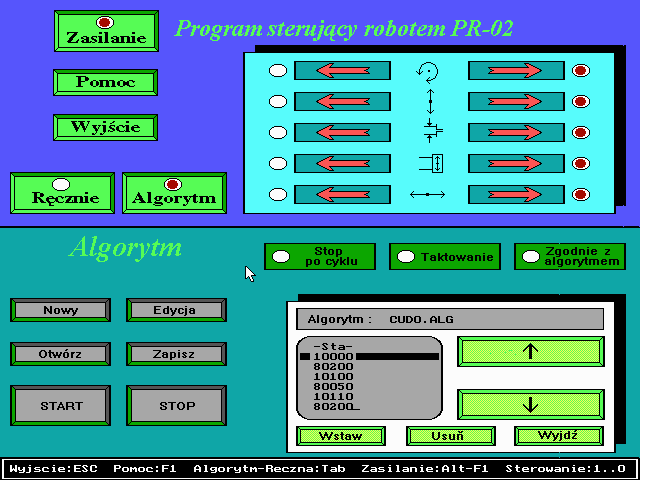
\includegraphics[width=\textwidth]{img/kolorowykwiatek.png}
			\caption{Oprogramowanie sterujące robotem}
		\end{figure} \noindent
	\section{Sterowanie ręczne}
		Z początku ćwiczenia zrealizowaliśmy sterowanie robota ręcznie. Miało to na celu zapoznanie się z czasami potrzebnymi do wykonania danego ruchu oraz funkcjonalnością poszczególnych przycisków. Następnie przystąpiliśmy do zastosowania implementacji wybranego przez nas programu sterującego.
	\section{Program sterujący}
		Ze względu na sugestię prowadzącego stworzyliśmy program sterujący działający na zasadzie opóźnień czasowych -- opcja potwierdzenia nie działała do końca tak jak należy.
		\\ \\
		Działanie programu sprowadza się do dokonywania przemieszczenia ramienia robota, a następnie odczekania czasu potrzebnego dla dokonania tego przemieszczenia.
\lstset{language=Matlab} 
\begin{lstlisting}[frame=single, keepspaces=true] 
PR-19
10000
80200
10100
80050
10110
80200
10010
80100
10000
00000
80200
00001
80200
00101
80050
00100
80050
00000
80050
\end{lstlisting}
		Powyższy program realizuje ruch obrotu, opuszczenia ramienia po przedmiot, złapanie przedmiotu, podniesienie go, obrót do poprzedniej pozycji, wyciągnięcie ramienia i odstawienie przedmiotu w danym miejscu. Następnie cofa ramię do pozycji początkowej. 
	\section{Wnioski}
		Ćwiczenie te przybliżyło nam zasady działania układu otwartego wraz z jego wadami -nie jesteśmy w stanie precyzyjnie określić położenia robota. Zapoznaliśmy się również z robotami pneumatycznymi, a nieszczelności w robocie pokazały nam jak się taki robot zachowuje w sytuacji uciekającego powietrza.
\end{document}